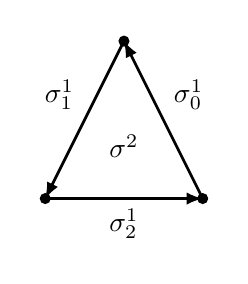
\begin{tikzpicture}[>=latex]
  % Coords
  \coordinate (V0) at (0,0);
  \coordinate (V1) at (2,0);
  \coordinate (V2) at (1,2);
  % Arrows\tilde{\sigma}
  \draw[line width=1pt, ->]
    (V0) -- node[below] {\( \sigma^{1}_{2} \)} (V1);
  \draw[line width=1pt, ->]
    (V1) -- node[above right] {\( \sigma^{1}_{0} \)} (V2);
  \draw[line width=1pt, ->]
    (V2) -- node[above left] {\(\sigma^{1}_{1}  \)} (V0);
  % Points
  \fill (V0) circle (2pt);
  \fill (V1) circle (2pt);
  \fill (V2) circle (2pt);
  % center
  \coordinate (C) at (1,0.666);
  \node at (C) {\( \sigma^{2} \)};

  \useasboundingbox ([shift={(1mm,1mm)}]current bounding box.north east) rectangle ([shift={(-1mm,-1mm)}]current bounding box.south west);
\end{tikzpicture}

